\documentclass[11pt]{book}
\usepackage{fontspec}
\setmainfont{TeX Gyre Pagella}
\usepackage[margin=1in]{geometry}
\usepackage{xcolor}
\usepackage{tikz}
\usetikzlibrary{arrows.meta}
\usepackage{amssymb}
\usepackage{enumitem}
\usepackage{titlesec}

\titleformat{\chapter}[display]{\bfseries\Large}{Sproll 01}{0.5em}{\Huge}
\titleformat{\section}{\bfseries\large}{\thesection}{0.6em}{}

\newenvironment{algorithmproc}[1]{%
\vspace{0.6em}\noindent\rule{\linewidth}{0.6pt}\\[0.2em]\textbf{How to Tell: #1}\\[0.3em]}%
{\\[0.2em]\noindent\rule{\linewidth}{0.6pt}\vspace{0.6em}}

\newenvironment{practicenow}{%
\vspace{0.6em}\noindent\rule{\linewidth}{0.6pt}\\[0.2em]\textbf{Practice Now}\\[0.3em]}%
{\\[0.2em]\noindent\rule{\linewidth}{0.6pt}\vspace{0.6em}}

\newenvironment{exercisebox}[1]{%
\vspace{0.8em}\noindent\rule{\linewidth}{0.6pt}\\[0.2em]\textbf{Exercises: #1}\\[0.3em]%
\begin{enumerate}[label=\arabic*., itemsep=0.4em]}%
{\end{enumerate}\noindent\rule{\linewidth}{0.6pt}\vspace{0.6em}}

\newenvironment{trythis}{%
\vspace{0.6em}\noindent\rule{\linewidth}{0.6pt}\\[0.2em]\textbf{Try This}\\[0.3em]}%
{\\[0.2em]\noindent\rule{\linewidth}{0.6pt}\vspace{0.6em}}

\newenvironment{summarybox}{%
\vspace{0.6em}\noindent\rule{\linewidth}{0.6pt}\\[0.2em]\textbf{What We Learned}\\[0.3em]}%
{\\[0.2em]\noindent\rule{\linewidth}{0.6pt}\vspace{0.6em}}

\begin{document}
\begin{titlepage}
\centering
\vspace*{1.4in}
{\Huge \textbf{SPROLL 01}}\\[0.5in]
{\huge Something Happened}\\[0.8in]
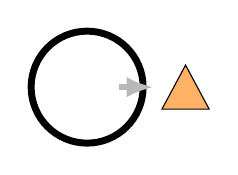
\begin{tikzpicture}
\draw[line width=2.5pt] (-1,0) circle (0.28in);
\draw[fill=orange!60] (-0.05,-0.28) -- (0.25,0.28) -- (0.55,-0.28) -- cycle;
\draw[-{Latex[length=3.5mm]}, line width=2pt, gray!55] (-0.6,0) -- (-0.15,0);
\end{tikzpicture}\\[0.8in]
{\Large The Sproll Curriculum}\\[0.2in]
{\large Cycle I: Pops --- Things, Differences, and Counting}
\end{titlepage}

\tableofcontents

\chapter*{Before You Begin}
\addcontentsline{toc}{chapter}{Before You Begin}

Sproll 00 was about telling one thing apart from another. It never asked you to choose anything; it only asked you to notice. This workbook asks something new. It asks what happens the moment you stop merely noticing several possible things and actually pick one of them.

That moment turns out to matter more than it might seem. Once you choose, something changes that cannot be undone by simply changing your mind: a fact now exists that did not exist a moment before. This workbook is about that moment, what mathematicians and computer scientists call a commitment, and about a word this curriculum uses for it from here on: a Pop.

\chapter{Choosing From What Could Happen}

\section{Several Ways to Go}

Imagine you are standing in front of three unlabeled doors. Nothing tells you what is behind any of them. Until you open one, all three are, as far as you know, equally possible outcomes. The moment you actually open one, though, something is different. You now know what is behind that door, and, just as importantly, the other two doors are no longer the one you opened. Something happened that cannot be taken back, even if you are allowed to open the other doors afterward.

Here is a simpler version of the same idea, without any doors.

\begin{center}
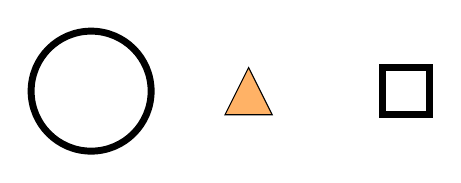
\begin{tikzpicture}
\draw[line width=2.5pt] (-2,0) circle (0.3in);
\draw[fill=orange!60] (-0.3,-0.3) -- (0,0.3) -- (0.3,-0.3) -- cycle;
\draw[line width=2.5pt] (1.7,-0.3) rectangle (2.3,0.3);
\end{tikzpicture}
\end{center}

Before anything happens, there are three ways to go: the circle, the triangle, or the square. None of them has happened yet. All three are available. Now suppose you choose the triangle.

\begin{center}

\begin{tikzpicture}
\draw[line width=1.5pt, gray!45] (-2,0) circle (0.3in);
\draw[fill=orange!60, line width=3.5pt] (-0.3,-0.3) -- (0,0.3) -- (0.3,-0.3) -- cycle;
\draw[line width=1.5pt, gray!45] (1.7,-0.3) rectangle (2.3,0.3);
\end{tikzpicture}
\end{center}

The triangle is now bold, because it is the one you chose. The circle and the square are faded, not because they have been erased or forgotten, but because they are no longer the thing that happened. You can still talk about them; you can still say ``I could have chosen the circle instead.'' What has changed is that only the triangle is now part of what actually took place.

This curriculum has a name for this kind of choosing: a \textbf{Pop}. A Pop is not just any object. It is the specific act of selecting one possibility from several available ones, so that afterward there is a fact, this one happened, where before there was only a list of things that might.

\begin{algorithmproc}{Is This a Pop?}
Ask three questions. First, before this moment, were there genuinely several different things that could have happened? Second, did something, a person, a machine, a rule, select exactly one of them? Third, after this moment, is it now a fact, not just a guess or a hope, that this one happened rather than the others? If all three answers are yes, you have found a Pop.
\end{algorithmproc}

\begin{practicenow}
Think of a recent moment when you chose one thing out of several options, ordering food, picking a book off a shelf, choosing a route to walk. Walk through the three questions in the box above and confirm that your example really was a Pop.
\end{practicenow}

\section{A Pop Is Not the Object Itself}

It is tempting to think a Pop just means ``the triangle,'' as though the word were simply another name for the shape you ended up with. That would be a mistake worth catching early, because this curriculum depends on the difference. The triangle by itself, sitting alone on a page, is not a Pop. A Pop is the event of choosing the triangle out of the circle, triangle, and square. The very same triangle, if it had simply been the only shape on the page from the start, with no other options ever available, would not be an example of a Pop at all, because nothing was chosen; there was nothing else it could have been instead.

\begin{exercisebox}{Section 1.2}
\item A vending machine has only one item left in it. You press the button and that item comes out. Was this a Pop, in the sense defined in this workbook? Explain using the three questions from the algorithm box.
\item A different vending machine has five different snacks available, and you press the button for one of them. Was this a Pop? Explain the difference between this case and the previous one.
\item Describe, in your own words, why ``the triangle'' and ``choosing the triangle out of three shapes'' are not the same thing, even though a picture of the result might look identical in both cases.
\end{exercisebox}

\chapter{One History, Many Ways It Could Have Gone}

\section{Starting Over With the Same Options}

Suppose you go back to the very beginning, with all three shapes available again, exactly as before: the circle, the triangle, and the square, none of them chosen yet. This time, instead of choosing the triangle again, you choose the square.

\begin{center}

\begin{tikzpicture}
\draw[line width=1.5pt, gray!45] (-2,0) circle (0.3in);
\draw[fill=orange!60, line width=1.5pt, gray!45] (-0.3,-0.3) -- (0,0.3) -- (0.3,-0.3) -- cycle;
\draw[line width=3.5pt] (1.7,-0.3) rectangle (2.3,0.3);
\end{tikzpicture}
\end{center}

Nothing about the original three options changed between the first attempt and this one. The circle, triangle, and square were exactly as available the second time as the first. What changed was which one got chosen. This gives you two different records of what happened, called \textbf{histories}: the first history contains the fact ``the triangle was chosen,'' and the second history contains the fact ``the square was chosen.'' Both histories started from the same three possibilities. They ended differently only because a different choice was made at the same branching point.

This is worth sitting with, because it is easy to assume that starting conditions determine an outcome all by themselves. They do not. The three shapes did not decide which one would be chosen; the act of choosing did that, and the same starting point can lead to genuinely different histories depending on which choice is made.

\begin{algorithmproc}{Same Start, Different History}
Two histories share a starting point exactly when both begin from the same set of available possibilities, with nothing yet chosen. They become different histories exactly when, at some point after that shared start, a different option is selected. It is entirely possible, and completely ordinary, for two different histories to share a starting point and still end up nowhere near each other.
\end{algorithmproc}

\section{An Everyday Example: A Game Replayed}

Board games and card games make this idea concrete. Imagine playing a simple game twice, starting from the identical setup both times, same board, same pieces, same starting positions. If even one player makes a different move the second time through, the rest of the game can unfold completely differently, even though both games began from the exact same starting arrangement. Chess players sometimes study this on purpose: they set up the same opening position and explore several different histories branching out from it, to see how different early choices lead to very different games later on.

\begin{trythis}
Pick a simple game you know (tic-tac-toe works well). Play it once, writing down each move in order. Then start over from the very same empty board and play it again, but change your very first move. Compare the two games. At what point, if any, did the two histories start to look completely different from each other?
\end{trythis}

\begin{exercisebox}{Section 2.1}
\item Explain, using the doors example from Chapter 1, what it would mean to have ``two histories'' starting from the same three doors.
\item Two friends are given the same three flavors of ice cream to choose from. One picks chocolate; the other picks strawberry. Are these two different histories, in the sense of this workbook, even though both friends started with exactly the same three options? Explain.
\item Challenge: if there are three shapes to choose from, how many different one-choice histories are possible in total, starting from that same beginning? List them.
\end{exercisebox}

\chapter{Counting What Happened}

\section{Counting Choices, Not Just Objects}

So far, this workbook has focused on a single choice at a time. Now consider making two choices, one after another, and building up a small history out of both of them.

Suppose you are choosing an ice cream cone. First you choose a flavor of ice cream: say, you choose vanilla out of vanilla, chocolate, and strawberry. Then, separately, you choose a topping: say, you choose sprinkles out of sprinkles, nuts, and no topping at all. Two separate choices were made, one after the other, each with its own set of available options.

How many things happened? The temptation is to look at your finished ice cream cone and count objects: one scoop, some sprinkles, maybe two things sitting in front of you. But that is not what this workbook is asking. It is asking how many choices were made along the way to get there, which is a count of \emph{events}, not a count of objects on a plate.

In this case, two choices were made: choosing the flavor, and choosing the topping. That is true regardless of how many scoops or sprinkles end up on the cone itself. If you had instead chosen a triple-scoop cone with one single flavor decision covering all three scoops, that would still be one choice, even though there are three scoops of ice cream to look at afterward.

\begin{algorithmproc}{Counting Events}
To count how many things happened in a history, do not count the objects present at the end. Count the separate moments at which something was chosen from among several available options. Each such moment counts once, no matter how large or small its result turns out to be.
\end{algorithmproc}

\begin{practicenow}
Think of a short sequence of choices you made recently that involved at least two decisions, getting dressed, planning a short trip, building something out of blocks. List the choices in order, and count how many separate choice-moments there were. Then separately count how many physical objects were involved at the end, and confirm that the two numbers do not have to match.
\end{practicenow}

\section{Why This Distinction Matters}

It might seem like a small, technical point, counting choices instead of objects, but it becomes important later in this curriculum. Two histories can end up looking exactly alike, with the same objects visible at the end, while having taken a completely different number of choices, or a different order of choices, to get there. A later workbook in this series returns to this exact tension. For now, the important habit is simply learning to ask ``how many things were chosen,'' not just ``how many things do I see.''

\begin{summarybox}
A Pop is the act of choosing one possibility out of several available ones, after which a new fact exists that did not exist before. Two histories can start from the exact same possibilities and still end up completely different, depending only on which choice is made. Counting what happened means counting choice-moments, not counting the objects left behind afterward.
\end{summarybox}

\begin{exercisebox}{Section 3.1}
\item A recipe asks you to choose a type of flour, then separately choose a type of sweetener. How many choices were made? How many separate ingredients might end up in the finished food?
\item Describe a real situation in which the number of choices made and the number of objects you end up with are clearly different numbers.
\item Challenge: can you describe a situation where exactly one choice is made, but the choice itself involves picking among more than two options? Does the number of available options at the time of choosing affect how many things ``happened''?
\end{exercisebox}

\chapter*{Looking Ahead}
\addcontentsline{toc}{chapter}{Looking Ahead}

This workbook has treated each choice mostly on its own, and treated two-choice sequences only in terms of how many choices were made, not the order they were made in. But order might matter more than it first appears. If you make two choices, and someone later looks only at the final result, could they tell which choice happened first? Or could two completely different orders of choosing lead to a final picture that looks exactly the same, hiding the order entirely?

That is the question Sproll 02: What Happened First? takes up next.

\chapter*{For Parents and Teachers}
\addcontentsline{toc}{chapter}{For Parents and Teachers}

This workbook introduces the first formal primitive of the underlying system this curriculum is built on, without naming the system explicitly. In that system, a Pop is defined as a commitment: the selection of one option from an available set, after which that option is treated as historically real and the others as not chosen, though never erased or forgotten. This is deliberately distinguished throughout the workbook from merely noticing or distinguishing an object, which was Sproll 00's subject; a Pop requires that there were genuinely multiple live possibilities beforehand and that one of them was selected.

Chapter 2's branching material (the same starting point producing two different histories) anticipates a formal idea, that alternative continuations from a shared starting point are a distinct structure from an ordinary single sequence of events, which later workbooks in this series develop precisely. Chapter 3's distinction between counting events and counting objects is stated narrowly on purpose: this workbook does not claim that a number is, in general, a property of a history, only that the length of a specific sequence of choices can be counted. That broader claim is left for a much later workbook, once the child has seen the same number arise from several different kinds of situations and can be invited to notice the pattern rather than being told it in advance.

\end{document}
